\documentclass[nooutcomes]{ximera}
\author{Jim Talamo}
\newcommand{\RR}{\mathbb R}
\renewcommand{\d}{\,d}
\newcommand{\dd}[2][]{\frac{d #1}{d #2}}
\renewcommand{\l}{\ell}
\newcommand{\ddx}{\frac{d}{dx}}
\newcommand{\dfn}{\textbf}
\newcommand{\eval}[1]{\bigg[ #1 \bigg]}


\outcome{Use algebra to manipulate the integrand.}
\outcome{Determine when a function is a composition of two or more functions.}
\outcome{Calculate indefinite and definite integrals requiring substitutions.}
\outcome{Recognize common patterns in substitutions.}
\outcome{Evaluate indefinite and definite integrals through a change of variables.}

%I want a separate section that reviews the FTC

\title[Dig-In:]{A review of integration techniques}

\begin{document}
\begin{abstract}
  We review common techniques to compute indefinite and definite integrals.
\end{abstract}
\maketitle

In some sense, calculating derivatives is straightforward.  Most of the functions of interest are sums, scalar multiples, products, quotients, or compositions of common functions whose derivatives we can find.  A ``brute force" application of the sum, scalar multiple, product, quotient, and chain rules will eventually lead to a correct derivative.  Integration is more of an art form.  We often have to apply various techniques in order to write down a nice formula for the antiderivatives. We explore some of the common ones here.

\section{Preliminary algebraic simplification}


A good first step in attempting to compute antiderivatives involves simplifying the integrand first.  Doing so requires careful algebra.
\begin{example}
  Compute:
  \[
  \int (7-x^2)^2 \d x
  \]
  \begin{explanation}
   Note first that $(7-x^2)^2 \neq 49-x^4$; we need to expand the integrand by writing out $(7-x^2)(7-x^2)$:
    \[
    \int (7-x^2)^2 \d x  = \int \answer[given]{49 - 14x^2 + x^4} \d x
    \]
    It's now not difficult to finish the problem:
    \[
    \int (49 - 14x^2 + x^4) \d x = \answer[given]{49x - \frac{14 x^3}{3} + \frac{x^5}{5}} + C
    \]
  \end{explanation}
\end{example}


%\begin{example}
%Consider the indefinite integral $\int \sqrt{x}(x+1)^2 \d x$.  
%
%While it may be tempting, note that $\sqrt{x}(x+1)^2 \neq (\sqrt{x}(x+1))^2$ by order of operations (exponentiation comes first). Instead, we can expand $(x+1)^2 = \answer[given]{x^2+2x+1}$ and rewrite the integrand:
%
%\begin{align*}
%\int \sqrt{x}(x+1)^2 \d x &= \int x^{1/2} (x^2+2x+1) \d x \\
%&=  \int x^{5/2}+2x^{3/2}+x^{1/2} \d x \\
%&= \frac{2}{7} x^{7/2}+\frac{4}{5}x^{5/2}+\frac{2}{3}x^{3/2}+C
%\end{align*}
%
%\end{example}

 
\begin{example}
Consider the indefinite integral $\int \frac{2x^2-3}{2x^2} \d x$.  

While it may be tempting, note that $\frac{2x^2-3}{2x^2} \neq \frac{\cancel{2x^2}-3}{\cancel{2x^2}}$.  We can never simplify by cancelling terms over addition or subtraction in the denominator.  Instead, we can split the fraction up then simplify.
\begin{align*}
\int \frac{2x^2-3}{2x^2} \d x &=\int \frac{2x^2}{2x^2}-\frac{3}{2x^2} \d x \\
&=  \int 1+\frac{3}{2}x^{-2} \d x \\
&= x- \answer[given]{\frac{3}{2}x^{-1}}+C
\end{align*}

\end{example}

  
\section{Substitution}

Sometimes, it is helpful to try to recognize when an integral involves reversing the chain rule for differentiation. When an integrand involves a composition of a trigonometric, exponential, or power and another function, letting a new variable represent the inner function helps.

\begin{example}
Consider $\int 2x e^{x^2+1} \d x$.  

Note that no algebra will help us simplify the expression.  The only antidifferentiation formula we have regarding the exponential is $\int e^x \d x = e^x +C$.  Let's start by letting the exponent in the original integral be a new variable $u$:

Let $u= x^2+1$.  We now need to write everything in the integral in terms of this new variable.  Recalling that if $u = f(x)$, the differentials are related by $\d u = f'(x) \d x$, we can write $\d u = \answer[given]{2x} \d x$.

We thus find

\begin{image}
  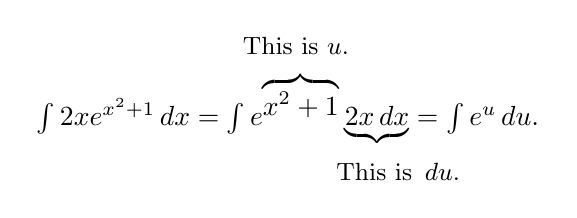
\begin{tikzpicture}
        \node at (0,0) {
          $\int 2x e^{x^2+1} \d x = \int e^{\overbrace{x^2+1}} \underbrace {2x \d x} = \int e^u \d u$.};
        \node at (1.4,-.8) {\small{This is $\d u$.}};
        
        \node at (.1,.8) {\small{This is $u$.}};
     
      \end{tikzpicture}
  \end{image}




The antiderivative in $u$ is now easy to compute.  

\[ \int e^u \d u = \answer[given]{e^u}+C \]

Reversing the substitution by setting $u=x^2+1$ above  now gives $\int 2xe^{x^2+1} \d x = e^{x^2+1}+C$.

\end{example}

\begin{remark}
Note that when we change the variable of integration, it is necessary to replace both the original variable and the differential.  That is, in the above example, we need to replace all $x$ terms with $u$ \emph{and} write $\d x$ in terms of $u$ and $\d u$. 
\end{remark}

In the last example, after letting $u$ be the exponent and transforming $\d x$, there were no $x$ terms left.  This does not always happen, but it does not mean that substitution does not aid in computing the indefinite integral.

\begin{example}
Compute $\int 4x \sqrt{2x+1} \d x$.

\begin{explanation}
Here, there is no preliminary algebra that will be helpful.  Since we have a square root of a function of $x$, we set $u=2x+1$ and find $\d u = \answer[given]{2} \d x$.  Thus:

\[
\int 4x \sqrt{2x+1} \d x = \int 4x \sqrt{u} \cdot  \frac{\d u}{2} =  \int 2x \sqrt{u} \d u
\]

Note that we now have an extra $x$ term in the integrand.  Since $x$ depends on $u$, we cannot move it outside of the integral.  Before abandoning hope that our substitution is useful here, we can ask whether it is easy to express this leftover $x$ in terms of $u$.  

Since $u= 2x+1$, we find that $x = \answer[given]{\frac{1}{2}(u-1)}$, so we can now rewrite the integral as:

\[
\int 4x \sqrt{2x+1} \d x =  \int 2x \sqrt{u} \d u = \int 2 \cdot \frac{1}{2}(u-1) \sqrt{u} \d u = \int (u-1)\sqrt{u} \d u
\]

We can now perform some algebra, then integrate.

\[
 \int (u-1)\sqrt{u} \d u = \int \left(u^{3/2} - u^{1/2} \right) \d u = \answer[given]{\frac{2}{5} u^{5/2} - \frac{2}{3} u^{3/2}} +C
\]
Substituting $u=2x+1$ to obtain the antiderivatives in terms of $x$, we find that

\[
\int 4x \sqrt{2x+1} \d x =  \frac{2}{5} (2x+1)^{5/2} - \frac{2}{3} (2x+1)^{3/2} +C.
\]
\end{explanation}
\end{example}


%Sometimes, the substitutions involve some preliminary algebra:
%
%\begin{example} 
%
%  Letting $a>0$, compute:
%  \[
%  \int \frac{1}{\sqrt{a-x^2}} \d x
%  \]
%  \begin{explanation}
%    Looking over our basic integral formulas, we see that this is similar to
%    \[
%    \int \frac{1}{\sqrt{1-x^2}}\d x= \answer[given]{\arcsin(x)}+C.
%    \]
%    So our goal will be to somehow ``transform'' the integral we are
%    trying to compute to one that is similar to the one we know how to
%    compute. First note:
%    \[
%    \int \frac{1}{\sqrt{a-x^2}} \d x  =
%    \int \frac{1}{\sqrt{\answer[given]{a}\left(1-\frac{x^2}{a}\right)}} \d x
%    \]
%    and since $a>0$, we may write:
%    \[
%    \int \frac{1}{\sqrt{a\left(1-\frac{x^2}{a}\right)}} \d x=
%    \int \frac{1}{\answer[given]{\sqrt{a}}\cdot \sqrt{1-\left(\frac{x}{\sqrt{a}}\right)^2}} \d x
%    \]
%    Recalling that we may always pull constants out of integrals, write:
%    \[
%    \int \frac{1}{\sqrt{a}\cdot \sqrt{1-\left(\frac{x}{\sqrt{a}}\right)^2}} \d x = 
%    \answer[given]{\frac{1}{\sqrt{a}}}\int \frac{1}{\sqrt{1-\left(\frac{x}{\sqrt{a}}\right)^2}} \d x 
%    \]
%    Ah! Now our integral looks more like one we can do. We will now
%    proceed using substitution. Set $u = \frac{x}{\sqrt{a}}$, and write with me
%    \begin{align*}
%      \d u &= \frac{\d x}{\sqrt{a}},\\
%      \d x &= \sqrt{a}\d u,
%    \end{align*}
%    and now
%    \begin{align*}
%    \frac{1}{\sqrt{a}}\int \frac{1}{\sqrt{1-\left(\frac{x}{\sqrt{a}}\right)^2}} \d x &=
%    \frac{1}{\sqrt{a}}\int \frac{1}{\sqrt{1-u^2}} \sqrt{a} \d u\\
%    &=\int \frac{1}{\sqrt{1-u^2}}\d u\\
%    &=\arcsin(u) + C\\
%    &=\arcsin\left(\frac{x}{\sqrt{a}}\right) + C.
%    \end{align*}
%  \end{explanation}
%\end{example}
%
%%%%EXERCISE: WHY NOT A COMPUTER? \int x(x+1)^50%%%%
%
%
%
%\begin{question}
%  Letting $a$ be nonzero, what is the antiderivative of $\frac{1}{a +
%    x^2}$?
%  \begin{prompt}
%    \[
%    \int \frac{1}{a + x^2} \d x = \answer[given]{\frac{1}{\sqrt{a}} \arctan\left(\frac{x}{\sqrt{a}}\right)}+C
%    \]
%  \end{prompt}
%  \begin{hint}
%    Try to use the same procedure used in the example above.
%  \end{hint}
%\end{question}


Let's see another example involving a trickier substitution and a definite integral.  First, recall the substitution theorem for definite integrals:

\begin{theorem}[Integral Substitution Formula] 
If $u$ is differentiable on the interval $[a,b]$ and $f$ is
differentiable on the interval $[u(a),u(b)]$, then
\[
\int_a^b f'(u(x)) u'(x) \d x =\int_{u(a)}^{u(b)} f'(u) \d u.
\]
\end{theorem}

This may look difficult to read, but it really just reminds us that to work with definite integrals, we need to write the integrand, the differential, and the limits of integration in terms of the new variable.  

\begin{example}
Compute $\int_0^2 \frac{6x^2}{(x^3+1)^2} \d x$

\begin{explanation}
We begin by setting $u = \answer[given]{x^3+1}$.  We now have to write the limits of integration in terms of $u$ as well as express the differential $\d x$ in terms of $u$ and $\d u$.

For the limits of integration, note that when $x=0$, we have $u = (0)^3+1 = 1$.  Similarly, when $x=2$, $u=\answer[given]{9}$.

Since $u=x^3+1$, we find $\d u = \answer[given]{3x^2} \d x$.

We can now write our original integral in terms of $u$:

\[
\int_{x=0}^{x=2} \frac{6x^2}{(x^3+1)^2} \d x = \int_{u=\answer[given]{1}}^{u=\answer[given]{9}} \answer[given]{\frac{2}{u^2}} \d u
\]

We can now evaluate the integral:

\[
\int_{u=1}^{u=9} \frac{2}{u^2} \d u = \int_{u=1}^{u=9}2u^{-2} \d u = \eval{-2u^{-1}}_{u=1}^{u=9} = -\frac{2}{9} - (-2) = \frac{16}{9}
\]
\end{explanation}
\end{example}

%Of course, sometimes the substitutions can be more complicated.
%
%\begin{example}
%Compute:
%\[
%\int_0^{16} \sqrt{4 - \sqrt{x}} \d x
%\]
%\begin{explanation}
%To make the integral appear a little nicer, let us try the substitution
%\[
%u = \sqrt{x}.
%\]
%Then:
%\begin{align*}
%\d u &= \answer[given]{\frac{1}{2 \sqrt{x}}} \d x,\\
%\d x &= 2 \sqrt{x} \d u = 2u \d u,
%\end{align*}
%where we used the fact that $u=\sqrt{x}$ in the last equality.  So:
%\begin{align*}
%\int_{x=0}^{x=16} \sqrt{4 - \sqrt{x}} \d x &=  \int_{u=\answer[given]{0}}^{u=\answer[given]{4}} \answer[given]{2u \sqrt{4-u}} \d u.
%\end{align*}
%From here we now make the second (and more obvious) substitution
%\[
%v = 4-u.
%\]
%Then $u = 4-v$, and: 
%\begin{align*}
%\d v &= - \d u,\\
%\d u &= - \d v.
%\end{align*}
%So:
%\begin{align*}
%\int_{x=0}^{x=16} \sqrt{4 - \sqrt{x}} \d x &= \int_{u=0}^{u=4} 2u \sqrt{4-u} \d u  \\
%&= \int_{v=\answer[given]{4}}^{v=\answer[given]{0}} 2 (4-v) \sqrt{v} (-1) \d v  \\
%&= \int_{v=\answer[given]{4}}^{v=\answer[given]{0}} 2v^{\frac{3}{2}} - 8v^{\frac{1}{2}}  \d v  \\
%&= \eval{ \answer[given]{  \frac{4}{5} v^{\frac{5}{2}} -  \frac{16}{3} v^{\frac{3}{2}} }}_{4}^{0}  \\
%&=  \left( 0 - 0 \right) - \left(\frac{4}{5} (4)^{\frac{5}{2}} - \frac{16}{3} (4)^{\frac{3}{2}}  \right)   \\
%&= \frac{128}{3} - \frac{128}{5}   \\
%&= \frac{256}{15}.
%\end{align*}
%\end{explanation}
%\end{example}


%\section{Algebra to the rescue} <-----MOVE TO ANOTHER SECTION

%With substitution, and a little algebraic manipulation, one can
%compute more integrals. In what follows, we will work many examples.
%In each case below we will present a ``novel'' integral, and then use
%algebra and substitution to change the form of the integral to one
%we know.



%Functions consisting of products of the sine and cosine can be
%integrated by using substitution and trigonometric identities. These
%can sometimes be tedious, but the technique is straightforward. The
%basic idea in each case is to somehow take advantage of a
%trigonometric identity, usually the Pythagorean identity, or a
%power-reduction formula:
%\begin{description}\index{Pythagorean identity}\index{power-reduction!formula}
%\item[Pythagorean Identity] $\cos^2(x) + \sin^2(x) = 1$
%\item[Cosine Power-Reduction] $\cos^2(x)= \frac{1+\cos(2x)}{2}$\index{cosine power-reduction}
%\item[Sine Power-Reduction] $\sin^2(x) = \frac{1-\cos(2x)}{2}$\index{sine power-reduction}
%\end{description}

%We'll work some examples to demonstrate how to use these formulas.

%\begin{example}
%  Compute:
%  \[
%  \int (\cos(x)+\sin(x))^2\d x
%  \]
 % \begin{explanation}
 %   Let's start by expanding the integrand:
%    \begin{align*}
%      \int &(\cos(x)+\sin(x))^2 \d x\\
%      &= \int \answer[given]{\cos^2(x) + 2\cos(x)\sin(x) + \sin^2(x)} \d x
%    \end{align*}
 %   Now if we rearrange we can use the Pythagorean identity, write with me:
 %   \begin{align*}
 %     \int &\cos^2(x) + 2\cos(x)\sin(x) + \sin^2(x) \d x \\
%      &= \int \cos^2(x) + \sin^2(x) + 2\cos(x)\sin(x) \d x\\
 %     &= \int \answer[given]{1 + 2\cos(x)\sin(x)} \d x
  %  \end{align*}
%    Now we may set $g = \sin(x)$ and so
 %   \begin{align*}
 %     \d g &= \answer[given]{\cos(x)} \d x,\\
 %     \d x & = \frac{\d g}{\cos(x)},
%    \end{align*}
 %   and we find
 %   \begin{align*}
 %     \int 1 + 2\cos(x)\sin(x) \d x &= \int 1 \d x + \int 2g \d g\\
%      &= x + g^2 + C\\
%      &= x + \answer[given]{\sin^2(x)}+C.
 %   \end{align*}
%  \end{explanation}
%\end{example}

%\begin{comment}
%Let's see one more example with trigonometric functions:
%
%\begin{example}
%  Compute:
%  \[
%  \int \frac{\sin(x) + \cos^2(x)}{\csc(x)} \d x
%  \]
%  \begin{explanation}
%    To start, let's express everything in terms of sine and cosine:
%    \begin{align*}
%      \int \frac{\sin(x) + \cos^2(x)}{\csc(x)} \d x &= \int \frac{\sin(x) + \cos^2(x)}{\frac{1}{\sin(x)}} \d x\\
%      &= \int \sin^2(x) + \sin(x)\cos^2(x) \d x
%    \end{align*}
%    if we use our power-reduction formula above, we find
%    \[
%    \int \answer[given]{\frac{1-\cos(2x)}{2}}+ \sin(x)\cos^2(x) \d x
%    \]
%    Splitting this integral up we now have
%    \begin{align*}
%      \int &\answer[given]{\frac{1}{2}} \d x - \int \frac{\cos(2x)}{2}\d x + \int \sin(x)\cos^2(x) \d x  \\
%      &= \answer[given]{\frac{x}{2} - \frac{\sin(2x)}{4} - \frac{\cos^3(x)}{3}}+C.
%    \end{align*}
%  \end{explanation}
%\end{example}
%\end{comment}

\section{Splitting Up Fractions}

In a similar vein, if you have a rational function, it can help to separate the
integrand into several fractions.

\begin{example}
  Compute:
  \[
  \int \frac{6x-8}{1+x^2}\d x
  \]
 
  \begin{explanation}
    Note that the substitution $u= 1+x^2$ is tempting, but it only will help us with part of the integrand!  Write with me:
    \[ \int \frac{6x-8}{1+x^2}\d x = \int \frac{6x}{1+x^2}-\frac{8}{1+x^2} \d x \]
      
Using a substitution, $ \int \frac{6x}{1+x^2}\d x = \answer[given]{3 \ln(1+x^2)}$+C, and using the inverse tangent antidifferentiation formula, $ \int \frac{8}{1+x^2}\d x = \answer[given]{8 \arctan(x)}$+C.

Hence, $\int \frac{6x-8}{1+x^2}\d x =  \answer[given]{3 \ln(1+x^2)- 8 \arctan(x)}+C$
  \end{explanation}
\end{example}

\begin{example}
  Compute:
  \[
  \int \frac{\cos^2(x)+1}{3 \cos^2(x)}\d x
  \]
 
  \begin{explanation}
It may be tempting to try to cancel just the expressions involving $\cos^2(x)$, but we have to split up the entire numerator over the denominator.

    \begin{align*}
    \int \frac{\cos^2(x)+1}{3 \cos^2(x)}\d x &=  \int \frac{\cos^2(x)}{3 \cos^2(x)} +  \frac{1}{3 \cos^2(x)}\d x \\
    &= \int \frac{1}{3} + \frac{1}{3} \sec^2(x) \d x \\
    & = \answer[given]{\frac{1}{3}x+\frac{1}{3}\tan(x)}+C 
    \end{align*}
      
  \end{explanation}
\end{example}

\section{Final Thoughts}
Understanding how to integrate is highly dependent on having a good grasp on how to differentiate functions and being comfortable with algebra. The techniques presented here are not an exhaustive list.  In order to become proficient computing integrals, there is no substitute for practice.  
%\section{Other Techniques}
%Your old friend (or enemy!) long-division\index{long-division} can help too.
%
%\begin{example}
%  Compute:
%  \[
%  \int \frac{3x^2-17x +1}{x-5} \d x
%  \]
%  \begin{explanation}
%    Now we will use long-division. Write:
%    %%\[
%    %% x-5\,\begin{array}[b]{@{}r@{}r} 
%    %% \answer[given]{3x-2} &\\ 
%    %% \cline{1-1}
%    %% \Bigg)\begin{array}[t]{@{}l@{}} 3x^2-17x+1\\ 
%    %%   \answer[given]{3x^2-15x} \\ 
%    %%   \divrule{0}{8}  ~~~~~\answer[given]{-2x+1} \\
%    %%   ~~~~~\answer[given]{-2x+10}\\
%    %%   \divrule{5}{8}
%    %%   ~~~~~~~~~~\answer[given]{-9}
%    %% \end{array}
%    %% \end{array}
%    %% \]
%    \begin{center}%%BADBAD
%      \begin{tikzpicture}[]
%        \node at (0,0) {
%    $x-5\,\begin{array}[b]{@{}r@{}r} 
%    3x-2 &\\ 
%    \cline{1-1}
%    \Bigg)\begin{array}[t]{@{}l@{}} 3x^2-17x+1\\ 
%      3x^2-15x \\ 
%      \divrule{0}{8}  ~~~~~~~-2x+1 \\
%      ~~~~~~~-2x+10\\
%      \divrule{5}{8}
%      ~~~~~~~~~~~~~~~~~-9
%    \end{array}
%    \end{array}
%          $
%        };
%      \end{tikzpicture}
%    \end{center}
%    From this we see that
%    \begin{align*}
%      \int \frac{3x^2-17x +1}{x-5} \d x &= \int 3x-2 - \answer[given]{\frac{9}{x-5}}\d x\\
%      &= \frac{3x^2}{2} - 2x -9 \ln|x-5| +C
%    \end{align*}
%    %Why is the rendering wrong?
%  \end{explanation}
%\end{example}
%
%Finally, sometimes it helps to complete the square.\index{complete the square}
%
%\begin{example}
%  Compute:
%  \[
%  \int \frac{1}{x^2-17x +1}\d x
%  \]
%  \begin{explanation}
%    To start, let's complete the square in the denominator. Write with me:
%    \begin{align*}
%      \int &\frac{1}{x^2-17x +1} \d x \\
%      &=  \int \frac{1}{x^2-17x +\left(\frac{17}{2}\right)^2 + 1 - \left(\frac{17}{2}\right)^2} \d x\\
%      &=  \int \frac{1}{\left(\answer[given]{x-\frac{17}{2}}\right)^2 + 1 - \left(\frac{17}{2}\right)^2} \d x
%    \end{align*}
%    At this point set $u= x-\frac{17}{2}$, so $\d u = \d x$ and we have
%    \begin{align*}
%    \int &\frac{1}{u^2 + 1 - \left(\frac{17}{2}\right)^2} \d u \\
%    &= \frac{1}{\sqrt{1 - \left(\frac{17}{2}\right)^2}} \arctan\left(\frac{u}{\sqrt{1 - \left(\frac{17}{2}\right)^2}}\right)\\
%    &= \frac{1}{\sqrt{1 - \left(\frac{17}{2}\right)^2}} \arctan\left(\frac{\answer[given]{x-\frac{17}{2}}}{\sqrt{1 - \left(\frac{17}{2}\right)^2}}\right).
%    \end{align*}
%  \end{explanation}
%\end{example}
%
%As you can see, integration is often far more challenging than differentiation.  Concerted time and practice are needed to become familiar with the necessary technique or techniques required to evaluate antiderivatives.  As a final strategy, please, when you are learning, feel free to find
%the answer using a computer. While this may seem like ``cheating'' but you
%can gain insight from it as long as you make sure you understand how to obtain the answer! 
%\begin{quote}
%  \textbf{Always remember: Don't give up.}
%\end{quote}
\end{document}
